\documentclass[aspectratio=169,12pt]{beamer}
\usetheme{CSCS}

\graphicspath{{./figs/}}

% define footer text
\newcommand{\footlinetext}{Directive Based GPU programming course 2018}

% Select the image for the title page
\newcommand{\picturetitle}{cscs_images/cscs_entrance_painting.pdf}

\lstdefinestyle{shstyle}{
  basicstyle=\scriptsize\ttfamily,
  keywordstyle=\color{blue},
  stringstyle=\color{magenta},
  commentstyle=\itshape\color{cscsred},
  language=bash,
}

\newcommand\shinline[2][]{\lstinline[style=shstyle,basicstyle=\ttfamily,#1]!#2!}

% Please use the predifined colors:
% cscsred, cscsgrey, cscsgreen, cscsblue, cscsbrown, cscspurple, cscsyellow,
% cscsblack, cscswhite

\author{Vasileios Karakasis, CSCS}
\title{Profiling and Debugging}
\subtitle{Directive Based GPU programming course 2018}
\date{May 14--15, 2018}

\begin{document}

% TITLE SLIDE
\cscstitle

\begin{frame}{Overview}
  \large
  \begin{itemize}
  \item Why and where my code crashes?
    \vspace\baselineskip
  \item Why my code does not perform as ``expected''?
  \end{itemize}
\end{frame}

\begin{frame}{Debugging}
  OpenACC translates to CUDA code, so you may use the corresponding tools:
  \begin{itemize}
  \item \texttt{cuda-memcheck}: Check for memory erros and race conditions
  \item \texttt{cuda-gdb}: Debug the generated CUDA kernels
  \item \texttt{nvprof+nvvp}: Detailed performance profiling
  \end{itemize}

  Other CUDA-aware tools:
  \begin{itemize}
  \item Allinea DDT: Debug MPI, CUDA, OpenMP applications + memory checking
  \end{itemize}

  Compiler-related diagnostics:
  \begin{itemize}
  \item Code generation diagnostics
  \item PGI debugger (\texttt{pgdb})
  \item PGI profiler (\texttt{pgprof})
  \item CrayPAT profiler
  \end{itemize}

\end{frame}

\begin{frame}[fragile]{Debugging}{\texttt{cuda-memcheck}}
  \begin{lstlisting}[basicstyle=\ttfamily\tiny]
$ srun -n1 -Cgpu cuda-memcheck ./blur.openacc

========= Invalid __global__ read of size 8
=========     at 0x00000098 in blur_twice_gpu_nocopies_84_gpu(double*, double*, int, int)
=========     by thread (66,0,0) in block (8192,0,0)
=========     Address 0x10253e00210 is out of bounds
=========     Saved host backtrace up to driver entry point at kernel launch time
=========     Host Frame:/opt/cray/nvidia/default/lib64/libcuda.so (cuLaunchKernel + 0x2cd) [0x23ce3d]
=========     Host Frame:/apps/common/UES/pgi/18.4/linux86-64/18.4/lib/libaccn.so (__pgi_uacc_cuda_launch3 + 0x19cc) [0x16d6c]
=========     Host Frame:/apps/common/UES/pgi/18.4/linux86-64/18.4/lib/libaccn.so [0x17950]
=========     Host Frame:/apps/common/UES/pgi/18.4/linux86-64/18.4/lib/libaccn.so (__pgi_uacc_cuda_launch + 0x10f) [0x17a6f]
=========     Host Frame:/apps/common/UES/pgi/18.4/linux86-64/18.4/lib/libaccg.so (__pgi_uacc_launch + 0x1ac) [0x15dec]
=========     Host Frame:./blur.openacc [0x52a5]
=========     Host Frame:./blur.openacc [0x57df]
=========     Host Frame:/lib64/libc.so.6 (__libc_start_main + 0xf5) [0x206e5]
=========     Host Frame:./blur.openacc [0x3489]
  \end{lstlisting}
\end{frame}

\begin{frame}[fragile]{Debugging}{\texttt{cuda-gdb}}
  \small Compile with \texttt{-g -Mcuda=debug}
  \vfill
  \begin{lstlisting}[basicstyle=\ttfamily\tiny]
$ srun -n1 -u -Cgpu cuda-gdb ./blur.openacc

(cuda-gdb) b blur_openacc.cpp:86
Breakpoint 1 at 0x40542b: file ./blur_openacc.cpp, line 86.
(cuda-gdb) r
Starting program: /users/karakasv/Devel/openacc-training/solutions/shared/./blur.openacc
[Thread debugging using libthread_db enabled]
Using host libthread_db library "/lib64/libthread_db.so.1".
dispersion 1D test of length n = 1048580 : 8.00003MB
[New Thread 0x2aaab52b2700 (LWP 17350)]
[New Thread 0x2aaab54b3700 (LWP 17351)]
[Switching focus to CUDA kernel 0, grid 3, block (1,0,0), thread (0,0,0), device 0, sm 2, warp 0, lane 0]

Breakpoint 1, blur_twice_gpu_nocopies_84_gpu<<<(8193,1,1),(128,1,1)>>> (
    out=0x10253200000, in=0x10252800000) at blur_openacc.cpp:87
87              for (auto i = 0; i < n; ++i) {
  \end{lstlisting}
\end{frame}

\begin{frame}{Debugging}{Using DDT}
  \begin{figure}
    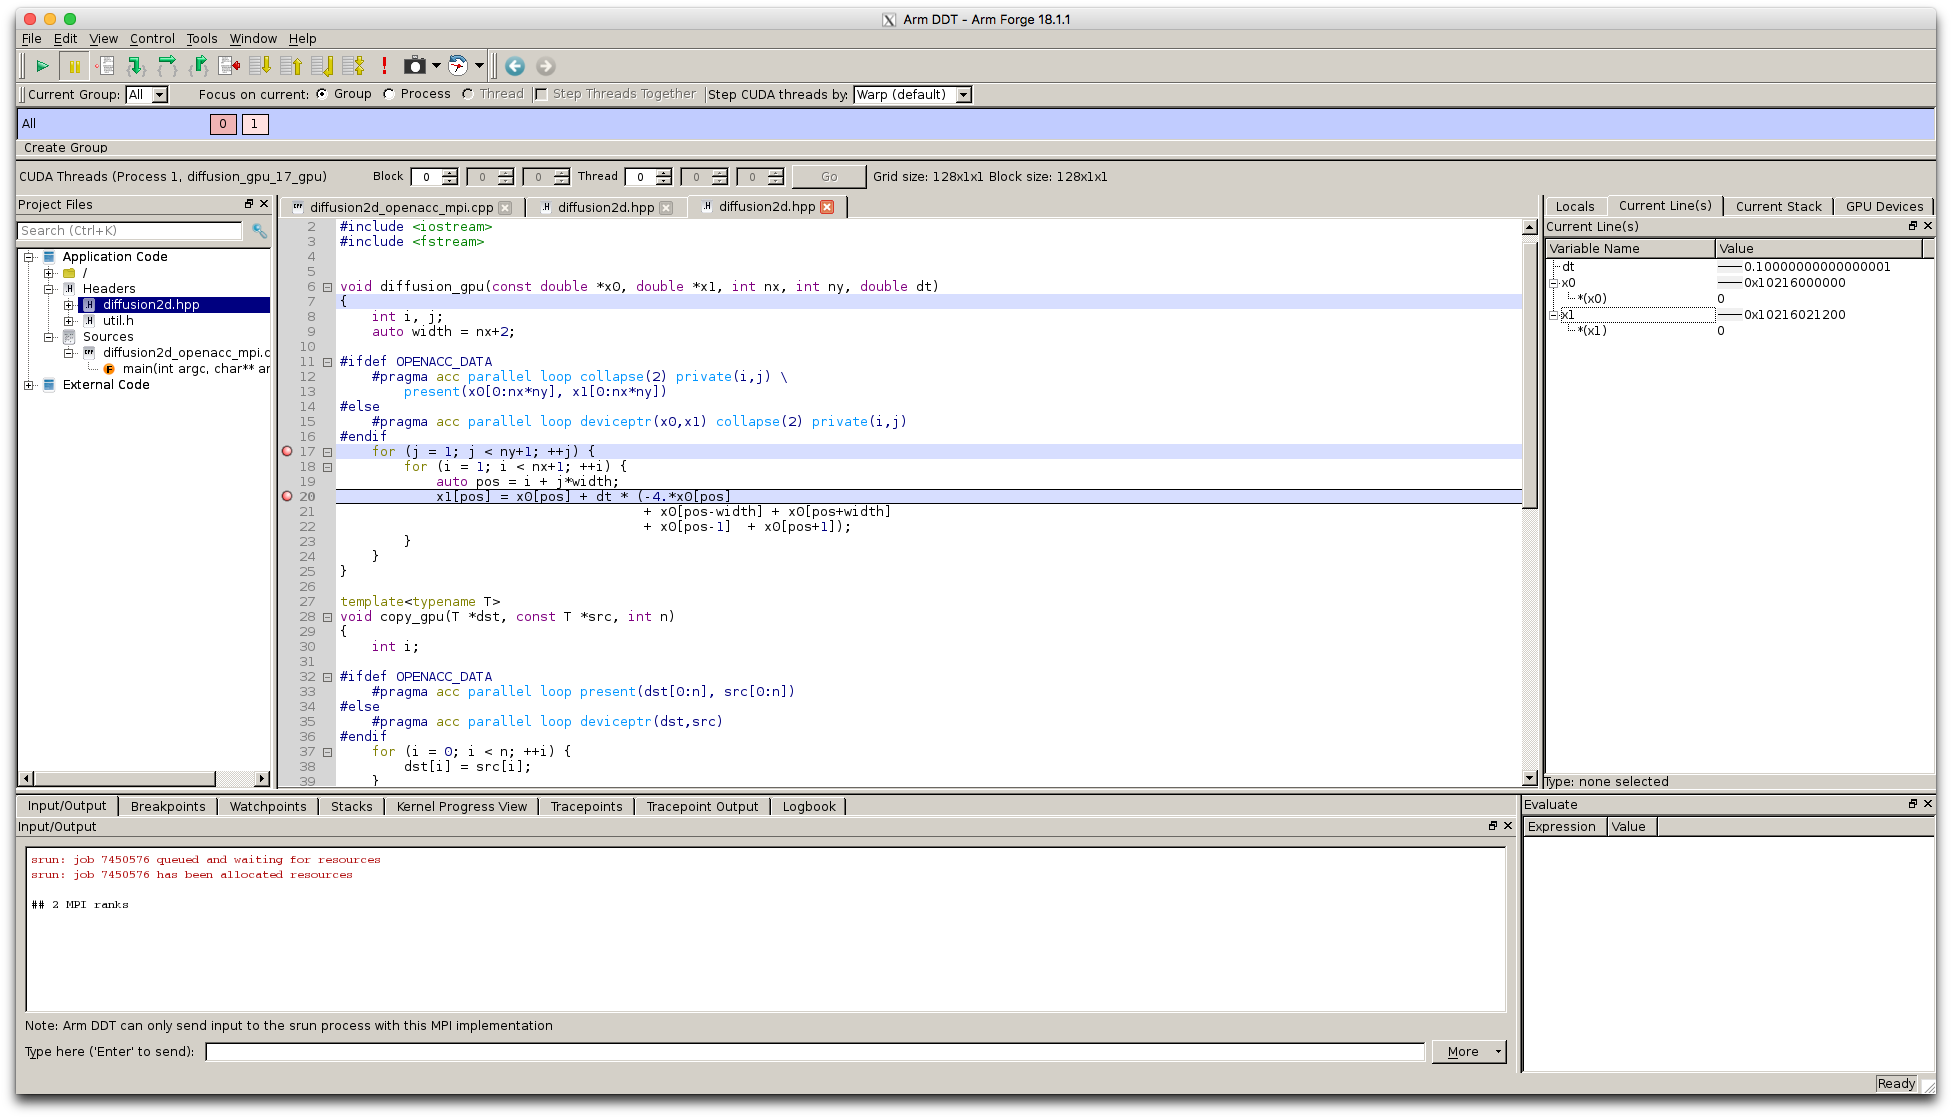
\includegraphics[width=\textwidth]{ddt.png}
  \end{figure}
\end{frame}

\begin{frame}{Profiling}{Using \texttt{nvprof} \& \texttt{nvvp}}
  \texttt{srun -N2 -Cgpu nvprof -o nvprof.\%h.\%p.out ./diffusion2d.openacc.mpi}
  \begin{figure}
    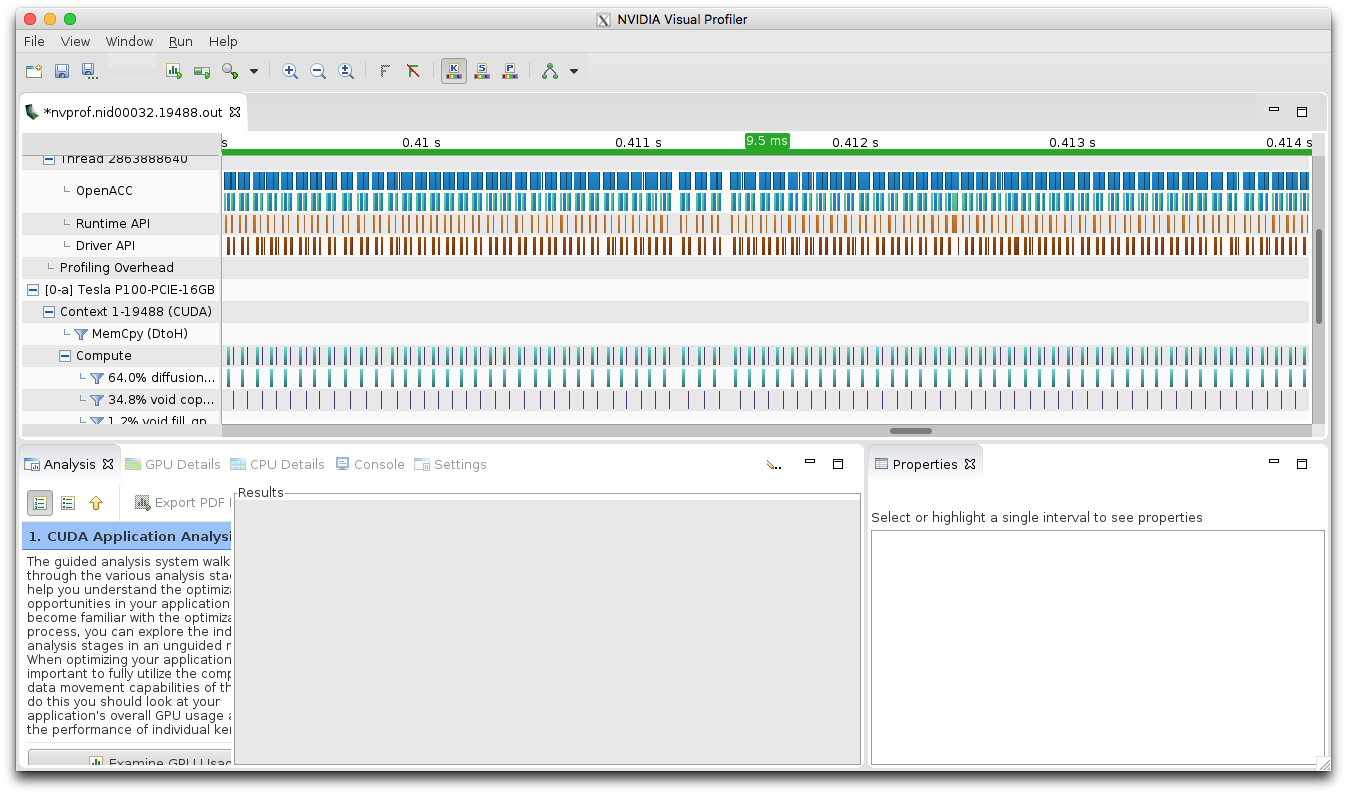
\includegraphics[width=.8\textwidth]{nvvp_timeline}
  \end{figure}
\end{frame}

\begin{frame}{Profiling}{Using \texttt{nvprof} \& \texttt{nvvp} -- Detailed analysis}
  \texttt{srun -N2 -Cgpu nvprof --analysis-metrics -o nvprof.\%h.\%p.out ./diffusion2d.openacc.mpi}
  \begin{figure}
    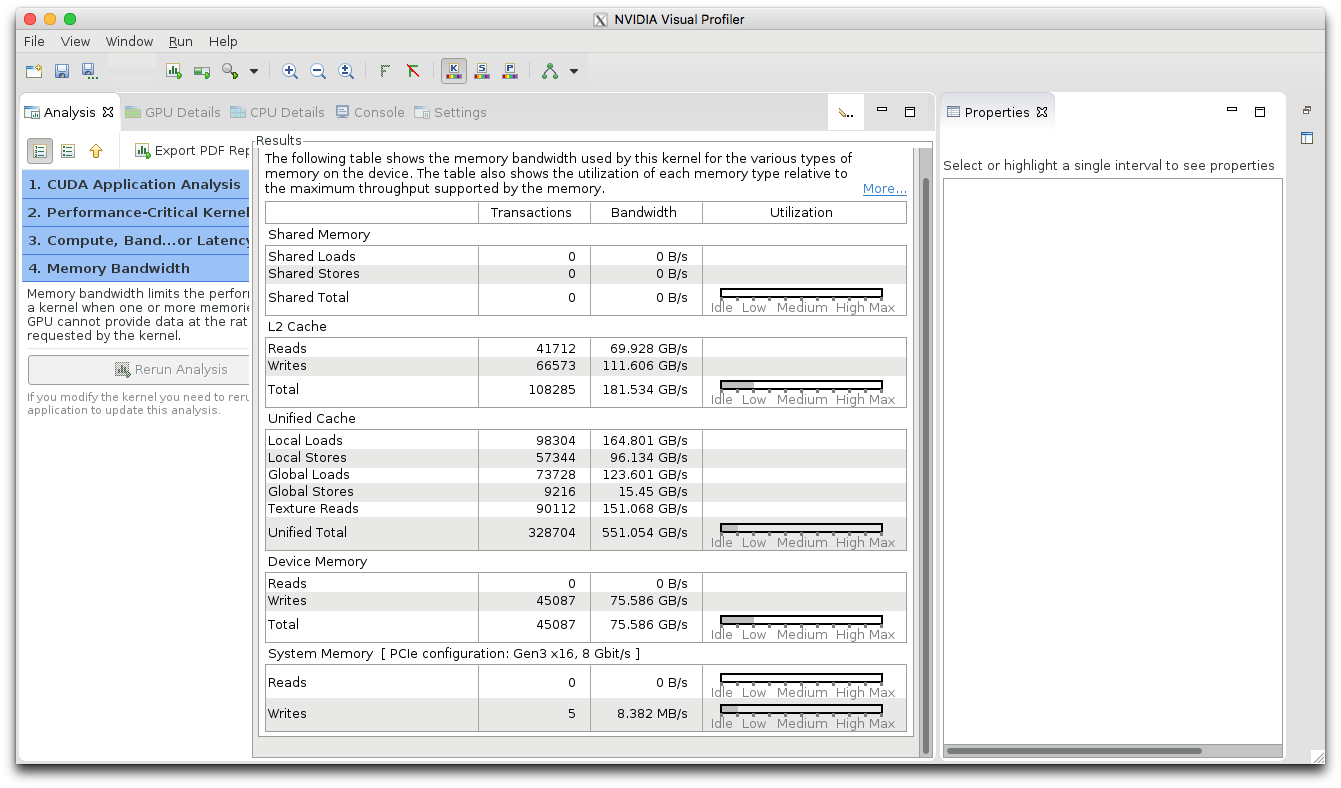
\includegraphics[width=.8\textwidth]{nvvp_membw}
  \end{figure}
\end{frame}

\begin{frame}[fragile]{Compiler diagnostics}{GPU kernel information}
  \begin{itemize}
  \item Compile with special flags (\texttt{-Minfo=accel} for PGI, \texttt{-hmsgs} for Cray)
  \end{itemize}

  \begin{lstlisting}[basicstyle=\ttfamily\tiny]
diffusion_gpu(const double *, double *, int, int, double):
      6, include "diffusion2d.hpp"
          17, Generating present(x0[:nx*ny],x1[:nx*ny])
              Accelerator kernel generated
              Generating Tesla code
              17, #pragma acc loop gang, vector(128) collapse(2) /* blockIdx.x threadIdx.x */
              18,   /* blockIdx.x threadIdx.x collapsed */
main:
     72, Generating create(x0[:buffer_size])
         Generating copyout(x1[:buffer_size])
void fill_gpu<double>(T1 *, T1, int):
      6, include "diffusion2d.hpp"
          53, Generating present(v[:n])
              Accelerator kernel generated
              Generating Tesla code
              53, #pragma acc loop gang, vector(128) /* blockIdx.x threadIdx.x */
  \end{lstlisting}
\end{frame}

\begin{frame}{}
  \large
  \begin{center}
    More during the hands-on!
  \end{center}
\end{frame}

\cscsthankyou{Thank you for your attention}

\end{document}
